%\documentclass[10pt]{article}
%\documentclass[crop,tikz,convert=pdf2svg]{standalone} %for an svg
\documentclass[%
  border={0pt 10pt 0pt 10pt}, % left bottom right top
  convert %=pdf2svg %for an svg
]{standalone}%

\usepackage{color}
\usepackage{tikz}
%%Source: https://dkumor.com/posts/technical/2018/08/15/causal-tikz/
% Tikz settings optimized for causal graphs.
% Just copy-paste this part
\usetikzlibrary{shapes,decorations,arrows,calc,arrows.meta,fit,positioning}
\tikzset{
    -Latex,auto,node distance =1 cm and 1 cm,semithick,
    state/.style ={ellipse, draw, minimum width = 0.7 cm},
    point/.style = {circle, draw, inner sep=0.04cm,fill,node contents={}},
    bidirected/.style={Latex-Latex,dashed},
    el/.style = {inner sep=2pt, align=left, sloped}
}
\begin{document}

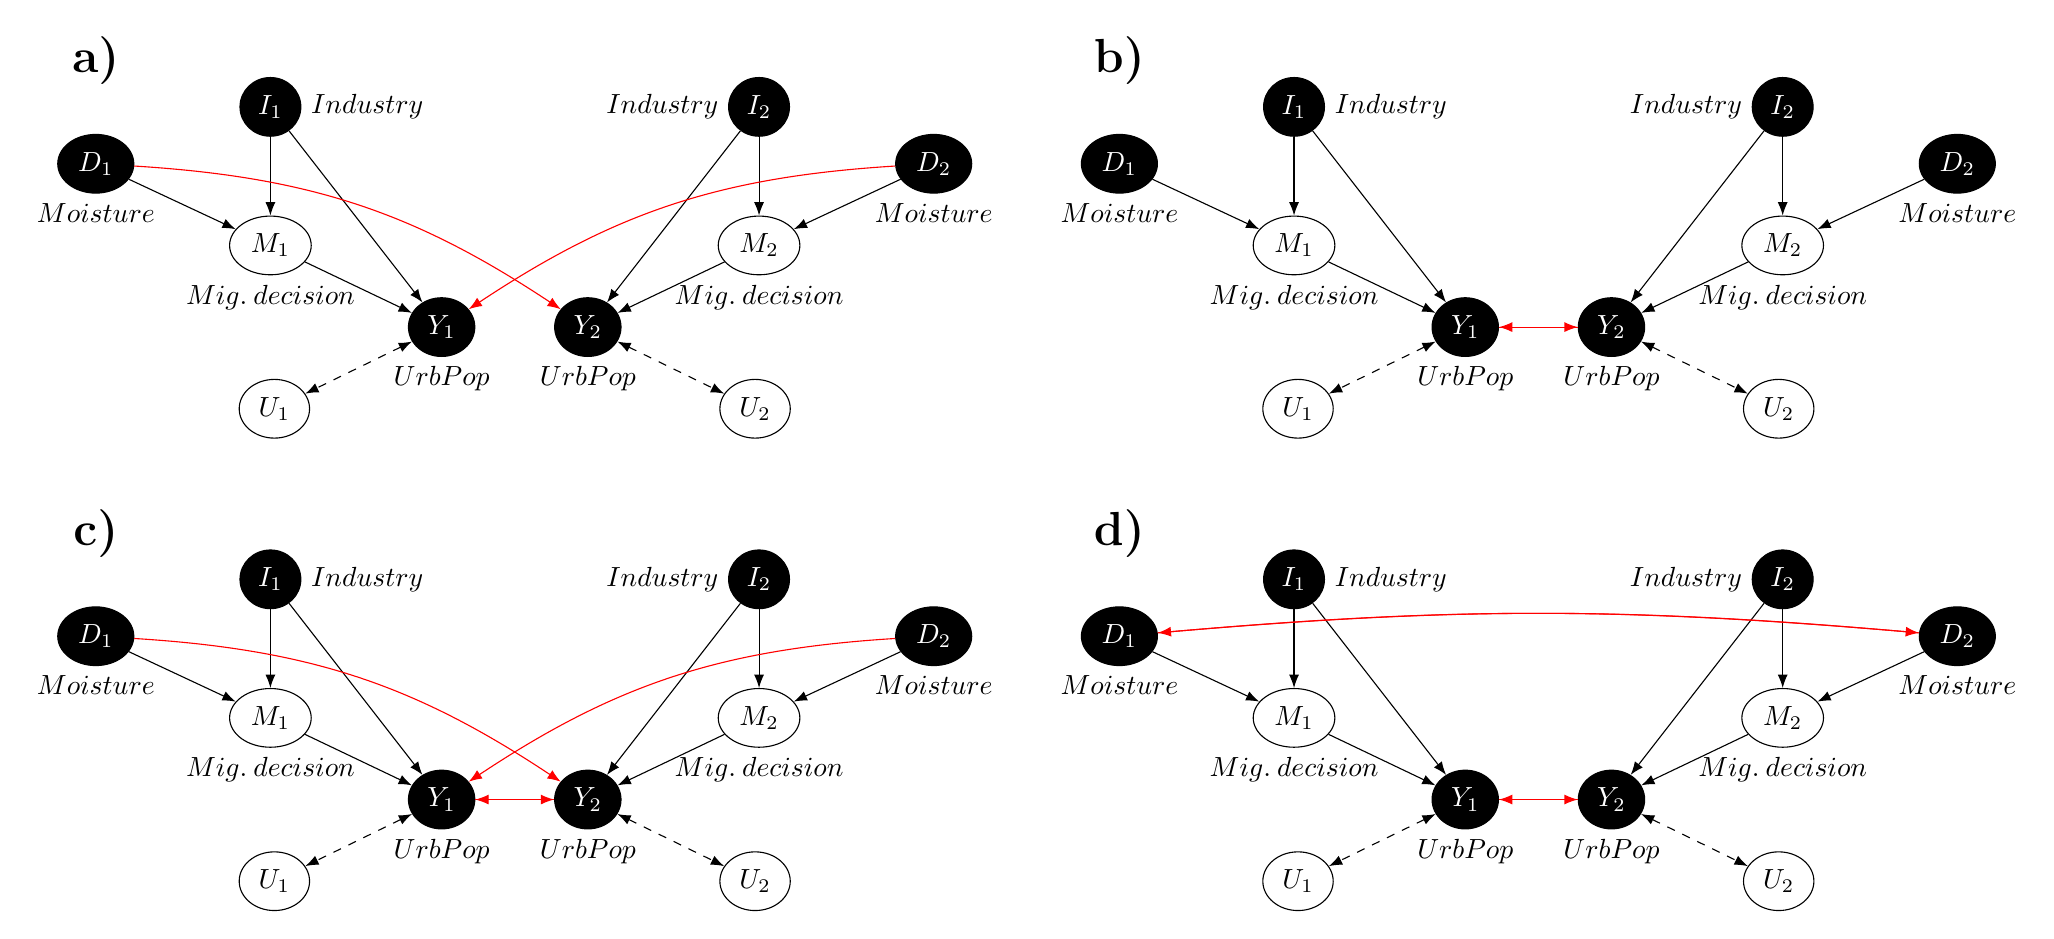
\begin{tikzpicture}
	%%% a
  	
    % Unit 1
    %%Background
    %\draw [rotate=-7, white, fill=orange!20] (-4.2,0) ellipse (4cm and 3.7cm);
    %\node (background1) at (-6,-0.5) {\textbf{\LARGE{Unit 1}}};
    
    %%Nodes
    \node[state, fill=black, text=white] (y1) at (-1,0) [label= below:$Urb Pop$] {$Y_1$};
    \node[state] (m1) [above left =of y1, yshift=-0.5cm, xshift=-0.5cm, label= below:$Mig. \: decision$] {$M_1$};
    \node[state, fill=black, text=white] (i1) [above =of m1, label= right:$Industry$] {$I_1$};
    \node[state, fill=black, text=white] (d1) [above left =of m1, yshift=-0.5cm, xshift=-0.5cm, label= below:$Moisture$] {$D_1$};
    \node[state] (u1) [below left =of y1, yshift=0.5cm, xshift=-0.5cm] {$U_1$};]
    
    % Unit 2
    %%Background
    %\draw [rotate=7, white,fill=green!20] (4.05,0) ellipse (4cm and 3.7cm);
    %\node (background1) at (6,-0.5) {\textbf{\LARGE{Unit 2}}};
    
    %%Nodes
    \node[state, fill=black, text=white] (y2) [right =of y1] [label= below:$Urb Pop$] {$Y_2$};
    \node[state] (m2) [above right =of y2, yshift=-0.5cm, xshift=0.5cm, label= below:$Mig. \: decision$] {$M_2$};
    \node[state, fill=black, text=white] (i2) [above =of m2, label= left:$Industry$] {$I_2$};
    \node[state, fill=black, text=white] (d2) [above right =of m2, yshift=-0.5cm, xshift=0.5cm, label= below:$Moisture$] {$D_2$};
    \node[state] (u2) [below right =of y2, yshift=0.5cm, xshift=0.5cm] {$U_2$};
    
    
    % Directed edge
    \path (m1) edge (y1);
    \path (i1) edge (m1);
    \path (i1) edge (y1);
    \path (d1) edge (m1);
    \path[bidirected] (y1) edge[] (u1);
    
    % Directed edge
    \path (m2) edge (y2);
    \path (i2) edge (m2);
    \path (i2) edge (y2);
    \path (d2) edge (m2);
    \path[bidirected] (y2) edge[] (u2);
    
    % connection D1 and D2
    \path[red] (d1) edge[bend left=15] (y2);
    \path[red] (d2) edge[bend right=15] (y1);

	%Title
	\node (background1) [above =of d1, yshift=-0.5cm] {\textbf{\LARGE{a)}}};  
   
   
    % ----------------------------------
    %% b
    
    % Unit 1
    %%Background
    %\draw [rotate=-7, white, fill=orange!20] (-4.2,0) ellipse (4cm and 3.7cm);
    %\node (background1) at (-6,-0.5) {\textbf{\LARGE{Unit 1}}};
    
    %%Nodes
    \node[state, fill=black, text=white] (y3) at (12,0) [label= below:$Urb Pop$] {$Y_1$};
    \node[state] (m3) [above left =of y3, yshift=-0.5cm, xshift=-0.5cm, label= below:$Mig. \: decision$] {$M_1$};
    \node[state, fill=black, text=white] (i3) [above =of m3, label= right:$Industry$] {$I_1$};
    \node[state, fill=black, text=white] (d3) [above left =of m3, yshift=-0.5cm, xshift=-0.5cm, label= below:$Moisture$] {$D_1$};
    \node[state] (u3) [below left =of y3, yshift=0.5cm, xshift=-0.5cm] {$U_1$};]
    
    % Unit 2
    %%Background
    %\draw [rotate=7, white,fill=green!20] (4.05,0) ellipse (4cm and 3.7cm);
    %\node (background1) at (6,-0.5) {\textbf{\LARGE{Unit 2}}};
    
    %%Nodes
    \node[state, fill=black, text=white] (y4) [right =of y3] [label= below:$Urb Pop$] {$Y_2$};
    \node[state] (m4) [above right =of y4, yshift=-0.5cm, xshift=0.5cm, label= below:$Mig. \: decision$] {$M_2$};
    \node[state, fill=black, text=white] (i4) [above =of m4, label= left:$Industry$] {$I_2$};
    \node[state, fill=black, text=white] (d4) [above right =of m4, yshift=-0.5cm, xshift=0.5cm, label= below:$Moisture$] {$D_2$};
    \node[state] (u4) [below right =of y4, yshift=0.5cm, xshift=0.5cm] {$U_2$};
    
    
    % Directed edge
    \path (m3) edge (y3);
    \path (i3) edge (m3);
    \path (i3) edge (y3);
    \path (d3) edge (m3);
    \path[bidirected] (y3) edge[] (u3);
    
    % Directed edge
    \path (m4) edge (y4);
    \path (i4) edge (m4);
    \path (i4) edge (y4);
    \path (d4) edge (m4);
    \path[bidirected] (y4) edge[] (u4);

    
    % connection Y1 and Y2
    \path[red] (y3) edge (y4);
    \path[red] (y4) edge (y3);

	%Title
	\node (background1) [above =of d3, yshift=-0.5cm] {\textbf{\LARGE{b)}}}; 
	
	
	
% ----------------------------------
    %% c
    
    % Unit 1
    %%Background
    %\draw [rotate=-7, white, fill=orange!20] (-4.2,0) ellipse (4cm and 3.7cm);
    %\node (background1) at (-6,-0.5) {\textbf{\LARGE{Unit 1}}};
    
    %%Nodes
    \node[state, fill=black, text=white] (y5) at (-1,-6) [label= below:$Urb Pop$] {$Y_1$};
    \node[state] (m5) [above left =of y5, yshift=-0.5cm, xshift=-0.5cm, label= below:$Mig. \: decision$] {$M_1$};
    \node[state, fill=black, text=white] (i5) [above =of m5, label= right:$Industry$] {$I_1$};
    \node[state, fill=black, text=white] (d5) [above left =of m5, yshift=-0.5cm, xshift=-0.5cm, label= below:$Moisture$] {$D_1$};
    \node[state] (u5) [below left =of y5, yshift=0.5cm, xshift=-0.5cm] {$U_1$};]
    
    % Unit 2
    %%Background
    %\draw [rotate=7, white,fill=green!20] (4.05,0) ellipse (4cm and 3.7cm);
    %\node (background1) at (6,-0.5) {\textbf{\LARGE{Unit 2}}};
    
    %%Nodes
    \node[state, fill=black, text=white] (y6) [right =of y5] [label= below:$Urb Pop$] {$Y_2$};
    \node[state] (m6) [above right =of y6, yshift=-0.5cm, xshift=0.5cm, label= below:$Mig. \: decision$] {$M_2$};
    \node[state, fill=black, text=white] (i6) [above =of m6, label= left:$Industry$] {$I_2$};
    \node[state, fill=black, text=white] (d6) [above right =of m6, yshift=-0.5cm, xshift=0.5cm, label= below:$Moisture$] {$D_2$};
    \node[state] (u6) [below right =of y6, yshift=0.5cm, xshift=0.5cm] {$U_2$};
    
    
    % Directed edge
    \path (m5) edge (y5);
    \path (i5) edge (m5);
    \path (i5) edge (y5);
    \path (d5) edge (m5);
    \path[bidirected] (y5) edge[] (u5);
    
    % Directed edge
    \path (m6) edge (y6);
    \path (i6) edge (m6);
    \path (i6) edge (y6);
    \path (d6) edge (m6);
    \path[bidirected] (y6) edge[] (u6);
      
    % connection Y1 and Y2
    \path[red] (y5) edge (y6);
    \path[red] (y6) edge (y5);
    \path[red] (d5) edge[bend left=15] (y6);
    \path[red] (d6) edge[bend right=15] (y5);
        
	%Title
	\node (background1) [above =of d5, yshift=-0.5cm] {\textbf{\LARGE{c)}}}; 
	
	
	    % ----------------------------------
    %% d
    
    % Unit 1
    %%Background
    %\draw [rotate=-7, white, fill=orange!20] (-4.2,0) ellipse (4cm and 3.7cm);
    %\node (background1) at (-6,-0.5) {\textbf{\LARGE{Unit 1}}};
    
    %%Nodes
    \node[state, fill=black, text=white] (y7) at (12,-6) [label= below:$Urb Pop$] {$Y_1$};
    \node[state] (m7) [above left =of y7, yshift=-0.5cm, xshift=-0.5cm, label= below:$Mig. \: decision$] {$M_1$};
    \node[state, fill=black, text=white] (i7) [above =of m7, label= right:$Industry$] {$I_1$};
    \node[state, fill=black, text=white] (d7) [above left =of m7, yshift=-0.5cm, xshift=-0.5cm, label= below:$Moisture$] {$D_1$};
    \node[state] (u7) [below left =of y7, yshift=0.5cm, xshift=-0.5cm] {$U_1$};]
    
    % Unit 2
    %%Background
    %\draw [rotate=7, white,fill=green!20] (4.05,0) ellipse (4cm and 3.7cm);
    %\node (background1) at (6,-0.5) {\textbf{\LARGE{Unit 2}}};
    
    %%Nodes
    \node[state, fill=black, text=white] (y8) [right =of y7] [label= below:$Urb Pop$] {$Y_2$};
    \node[state] (m8) [above right =of y8, yshift=-0.5cm, xshift=0.5cm, label= below:$Mig. \: decision$] {$M_2$};
    \node[state, fill=black, text=white] (i8) [above =of m8, label= left:$Industry$] {$I_2$};
    \node[state, fill=black, text=white] (d8) [above right =of m8, yshift=-0.5cm, xshift=0.5cm, label= below:$Moisture$] {$D_2$};
    \node[state] (u8) [below right =of y8, yshift=0.5cm, xshift=0.5cm] {$U_2$};
    
    
    % Directed edge
    \path (m7) edge (y7);
    \path (i7) edge (m7);
    \path (i7) edge (y7);
    \path (d7) edge (m7);
    \path[bidirected] (y7) edge[] (u7);
    
    % Directed edge
    \path (m8) edge (y8);
    \path (i8) edge (m8);
    \path (i8) edge (y8);
    \path (d8) edge (m8);
    \path[bidirected] (y8) edge[] (u8);
    
    % connection D1 and D2
    \path[red] (d7) edge[bend left=5] (d8);
    \path[red] (d8) edge[bend right=5] (d7);

    % connection Y1 and Y2
    \path[red] (y7) edge (y8);
    \path[red] (y8) edge (y7);

	%Title
	\node (background1) [above =of d7, yshift=-0.5cm] {\textbf{\LARGE{d)}}}; 
	

\end{tikzpicture}
\end{document}